%analisis del caso de estudio %
Como se vi\'o anteriormente las arquitecturas o marcos de trabajo que soporten consciencia contextual deben cumplir con ciertos requerimientos \cite{dey1999architecture}, para poder cubrir estas necesidades se necesita que el marco de trabajo sea accesible por el groupware desde cualquier ubicaci\'on, con esto se cubre la distribuci\'on de la arquitectura, as\'i la publicaci\'on de servicios web consumibles desde el sistema colaborativo se vuelve una soluci\'ona este problema, adem\'as de que con estos servicios aumenta la compatibilidad con otro tipo de plataformas al enviar sus mensajes serializados en Json o envueltos en una solicitud SOAP. Con estos servicios se hace posible la recepci\'on de informaci\'on contextual y la emisi\'on de los resultados hacia el groupware. Con la informaci\'on recivida se mantiene un registro de la actividad del groupware que puede ser \'util para an\'alisis futuros como miner\'ia de datos o reconocimiento de patrones.

La arquitectura no debe de estar enganchada a un escenario en particular, debe de funcionar tanto para un sistema de gu\'ia de turistas como para uno de oficina, es por eso que la definici\'on del modelo contextual se divide en dos partes, un meta modelo compuesto por entidades que describen una actividad mediante realciones de elementos tales como \textit{actores}, \textit{objetos}, \textit{tareas}, \textit{categor\'ias}, \textit{roles}, \textit{comunidades} y \textit{objetivos} con lo que se modela las interacciones del groupware, una vez modelado el dominio del sistema se instancia a partir del meta modelo, es en esta instanciaci\'on donde se guardar\'an los datos del groupware.

Los datos recibidos deben de ser gestionados en bases de datos y procesados por un motor de razonamiento, el cu\'al tiene que recibir informaci\'on contextual y mediante alg\'un proceso tiene que dar como resultado informaci\'on para el usuario o un comando de ejecuci\'on para el groupware. Una vez que se procesa la informaci\'on esta se tiene que preparar para su distribuci\'on en los diferentes dispositivos cliente. Para esto se debe de considerar que al ser las actividades colaborativas los usuarios pueden compartir el contexto en algunas ocasiones, de lo que se desprende la necesidad de agregar la informaci\'on contextual de usuarios que compartan ciertos atributos establecidos para una situaci\'on en particular, es decir, fusionar la informaci\'on de tales usuarios para un manejo de la informaci\'on m\'as eficiente.

\subsection{Caso de estudio}

Para el actual proyecto se necesita un groupware al cu\'al se le pueda acoplar la arquitectura para poder analizar sus datos, en este caso el sistema elegido es un videojuego colaborativo de disparos en primera persona, \textit{AssaultCube}. Este groupware en particular tiene las caracter\'isticas de ser distribuido y s\'incrono seg\'un la clasificaci\'on de Ellis\cite{ellis1991groupware}, contiene varios tipos de elementos y los modos multijugador son entre equipos en los cuales se requiere de una buena colaboraci\'on para cumplir los objetivos de la actividad, El juego cuenta con un servidor y varios clientes que se conect\'an a \'el para poder jugar, la arquitectura tendr\'a que estar acoplada al servidor ya que este es el que recibe toda la informaci\'on de las actividades de los clientes. \textit{Assault Cube} tiene diferentes modos de juego, entre ellos capturar la bandera, cuyo objetivo es llegar a la base enemiga y recuperar la bandera que est\'a ah\'i para regresarla a la propia bas; otro modo de juego es rey de la colina, que tiene por objetivo mantenerse m\'as tiempo en una posici\'on marcada por el juego que el equipo contrario; hay m\'as formas de juego adem\'as de estas dos, y en cada una de ellas las actividades son diferentes y poseen objetivos diferentes, sin embargo pueden compartir interacciones como eliminar a un enemigo por ejemplo.

\begin{figure}[h!]
\centering
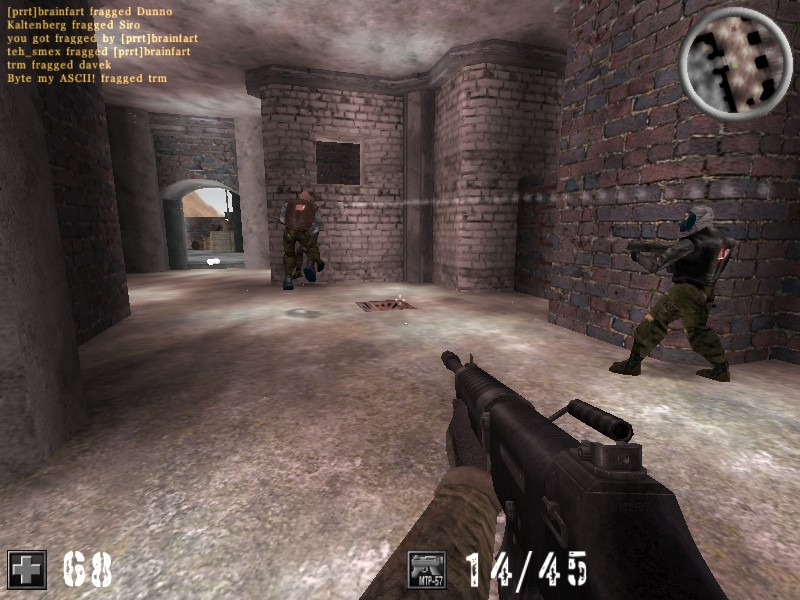
\includegraphics[scale=.15]{images/assaultcube}
\caption{Assault Cube}
\label{gw:asscb}
\end{figure}

En la Tabla 1 se muestran las interacciones identificadas en el juego para la actividad relacionada al modo de juego de capturar la bandera, estas interacciones est\'an relacionadas directamente con las actividades que se pueden llevar a cabo en el groupware, las interacciones se vuelven irrelevantes cuando no tienen conexi\'on con ninguna actividad, por ejemplo las interacciones del usuario con elementos de configuraci\'on en este caso particular, como en la interacci\'on \textit{"Jugador elige modo de juego"}. En estas interacciones se encuentran algunos elementos del modelo como pueden ser Actores, Tareas y Objetos,  esto nos da la pauta para empeazar a dise\~nar nuestro modelo.

\begin{center}
\label{AC:interacciones}
\begin{longtable}{|p{5cm}|p{7cm}|}

\caption{Tabla de interacciones detectadas en \textit{Assault Cube}}\\
\hline
\textbf{Interacci\'on} & \textbf{Elementos identificados}\\
\hline
\endfirsthead
\multicolumn{2}{c}%
{\tablename\ \thetable\ -- \textit{... Contin\'ua de p\'agina anterior}} \\
\hline
\textbf{Interacci\'on} & \textbf{Elementos identificados} \\
\hline
\endhead
\hline \multicolumn{2}{r}{\textit{Contin\'ua en siguiente p\'agina...}} \\
\endfoot
\hline
\endlastfoot
\textbf{Jugador se Mueve} & Actor: Jugador; Tarea: Moverse\\\hline

\textbf{Jugador salta} & Actor: Jugador; Tarea: Saltar\\\hline

\textbf{Jugador dispara arma} & Actor: Jugador; Tarea: Saltar; Objeto: Arma\\\hline

\textbf{Jugador recarga arma} & Actor: Jugador; Tarea: Recargar; Objeto: Arma\\\hline

\textbf{Jugador dispara arma} & Actor: Jugador; Tarea: Saltar; Objeto: Arma\\\hline

\textbf{Jugador cambia arma} & Actor: Jugador; Tarea: Cambiar; Objeto: Arma\\\hline

\textbf{Jugador obtiene mejora de salud} & Actor: Jugador; Tarea: Obtener; Objeto: Mejora de salud\\\hline

\textbf{Jugador obtiene protecci\'on} & Actor: Jugador; Tarea: Obtener; Objeto: Protecci\'on\\\hline

\textbf{Jugador obtiene munici\'on} & Actor: Jugador; Tarea: Obtener; Objeto: munici\'on\\\hline

\textbf{Jugador envia mensaje de texto} & Actor: Jugador; Tarea: enviar; Objeto: Mensaje de texto\\\hline

\textbf{Jugador envia mensaje de voz predefinido} & Actor: Jugador; Tarea: enviar; Objeto: Mensaje de voz\\\hline

\textbf{Jugador elige arma inicial} & Actor: Jugador; Tarea: Elegir; Objeto: Arma predeterminada\\\hline

\textbf{Jugador cambia rol} & Actor: Jugador; Tarea: Cambiar; Objeto: Rol\\\hline

\textbf{Jugador se agacha} & Actor: Jugador; Tarea: Agacharse\\\hline

\textbf{Jugador se suicida} & Actor: Jugador; Tarea: Suicidarse\\\hline

\textbf{Jugador es eliminado} & Actor: Jugador; Tarea: Ser eliminado\\\hline

\textbf{Jugador elimina oponente} & Actores: JugadorA, JugadorB; Tarea: Eliminar\\\hline

\textbf{Jugador reaparece} & Actor: Jugador; Tarea: Reaparecer\\\hline

\textbf{Jugador captura bandera} & Actor: Jugador; Tarea: Capturar; Objeto: Bandera\\\hline

\textbf{Jugador regresa bandera a su base} & Actor: Jugador; Tarea: Recuperar; Objeto: Bandera \\\hline

\textbf{Jugador ve mapa} & Actor: Jugador; Tarea: Ver; Objeto: Mapa\\\hline

\textbf{Jugador ve puntuaciones} & Actor: Jugador; Tarea: Ver; Puntuaciones\\\hline

\end{longtable}
\end{center}

En la lista anterior de interacciones se pueden identificar ya algunos elementos del modelo del groupware, por ejemplo, jugador como actor; arma, munici\'on y mapa como posibles objetos, y el conjunto de ellos relacionados con una acci\'on como tareas. Tambi\'en a partir de estas interacciones pueden empezar a definirse algunas reglas, por ejemplo establecer una regla que diga que si un jugador captur\'o una bandera y est\'a en peligro inminente de ser atacado, el sistema muestre a sus compa\~neros de equipo la ubicaci\'on del abanderado y env\'ie una se\~nal de auxilio para que ellos puedan acudir a su ayuda.

\subsection{Prototipo}
Para el presente trabajo se hace uso de un meta modelo contextual para el modelado de actividades de sistemas groupware basado un modelo propuesto anteriormente\cite{montane2013context}, en el cual se pueden encontrar dos categor\'ias de elementos, interactivos y cohesivos.  Entre los interactivos se encuentran \textit{actores}, que son los usuarios del sistema, \textit{objetos} que se usan en \textit{tareas} o que son producto de ellas, \textit{categor\'ias} que clasifican a los actores, objetos y tareas seg\'un sus atributos, por \'ultimo est\'an los roles del objeto y del actor los cuales son asignadas a una tarea para establecer el rol que va a tener el actor u objeto involucrado en dicha tarea. Entre los datos cohesivos se encuentran las \textit{comunidades} que son el conjunto de actores con una \textit{actividad} en com\'un, estas actividades pueden tener varias \textit{metas} las cuales se cumplen realizando tareas. Por \'ultimo se encuentran las reglas que son sentencias en un lenguaje definido para poder inferir las interacciones que suceden en el groupware. En la figura \ref{cmp:mmc} se muestra un diagrama de los elementos de este modelo y sus relaciones.

\begin{figure}[h!]
  \centering
    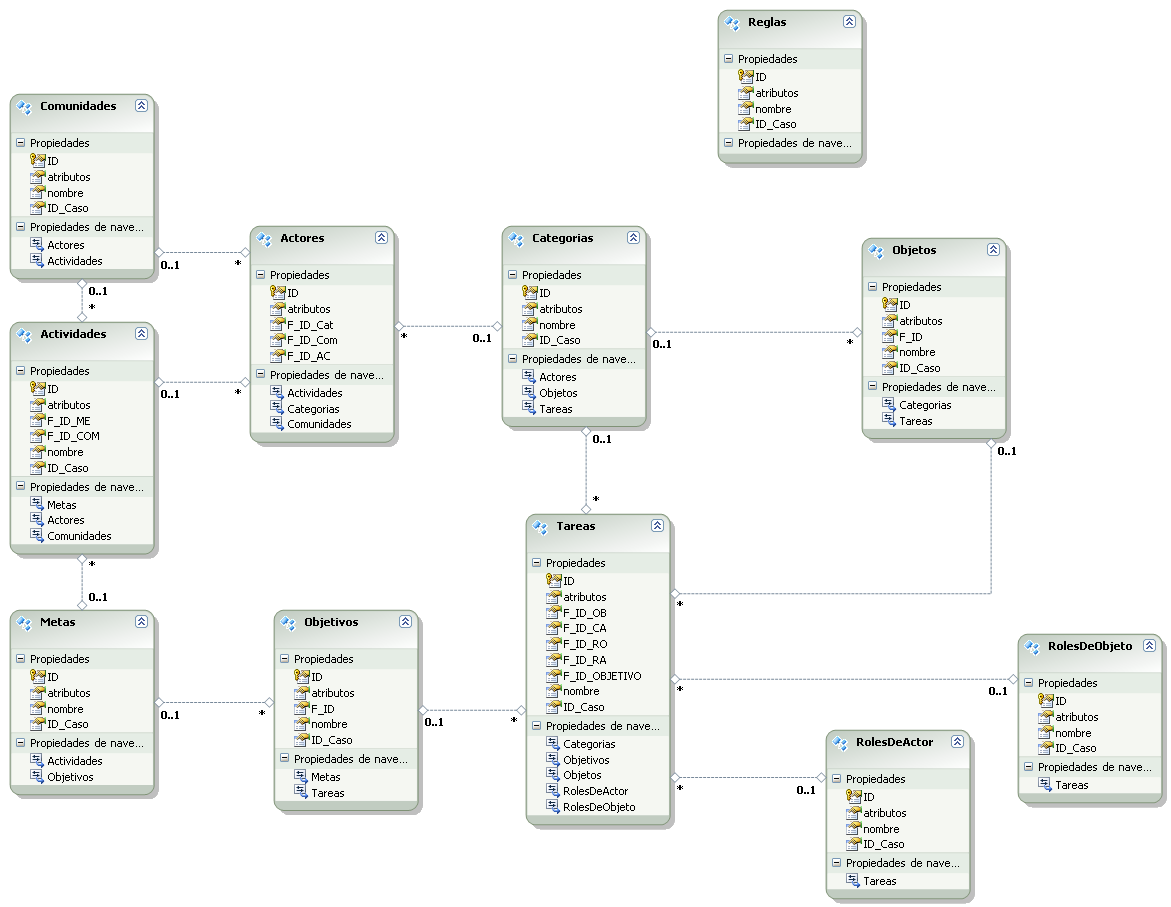
\includegraphics[scale=0.35]{images/modelo}
  \caption{Meta modelo contextual}
  \label{cmp:mmc}
\end{figure}

Con este meta modelo contextual se pueden describir groupwares definiendo cada uno de estos elementos a partir de interacciones, una vez dado de alta un caso junto con sus reglas se instancia un modelo que representar\'a al sistema colaborativo y almacenar\'a las variables contextuales que este transmita a la arquitectura. Cabe mencionar que en este metamodelo los elementos cuentan con 3 atributos principales, un identificador del objeto, un nombre descriptivo, y una lista de atributos almacenados en formato JSON, lo que vuelve flexible la forma de registrar casos de estudio.

La arquitectura que se propone mostrada en la figura \ref{ARCH:propuesta}, cuenta con tres capas: recuperaci\'on de datos, gesti\'on de contexto, y uso de contexto. Para poder acoplar la arquitectura primero se tiene que dar de alta un modelo del groupware. Para esto se cre\'o una plataforma para registrar casos de estudio en la que se establece el nombre del caso de estudio y todos sus elementos, una vez creado el meta modelo del groupware se instancia el modelo y se administran las interacciones para poder relacionar sus elementos, esto se hace en una segunda plataforma en la que se toman los elementos del meta modelo y se instancia uno m\'as apegado al groupware, ya con este modelo se pueden capturar los datos contextuales que el sistema va a enviar a la arquitectura. 

\begin{figure}[h!]
\centering
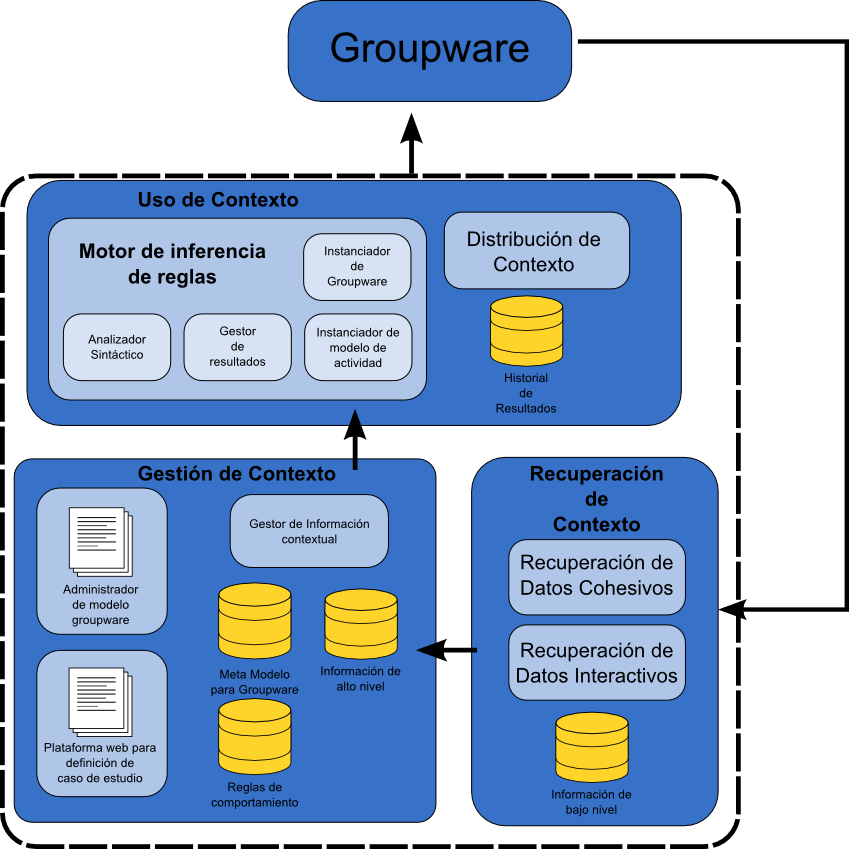
\includegraphics[scale=0.40]{images/arch2}
\caption{Arquitectura propuesta}
\label{ARCH:propuesta}
\end{figure}

La arquitectura, similar a la arquitectura en que se bas\'o, se divide en tres capas; la capa de recuperaci\'on de datos, la capa de gestion de datos y la capa de uso de contexto. En la primera capa, la de recuperac\'on de datos, se captura informaci\'on contextual enviada por el groupware por medio de servicios web publicados para la comunicaci\'on entre la arquitectura y el sistema, estos datos son enviados en un formato espec\'ifico para que capas superiores puedan procesarla. Seguido de este m\'odulo est\'a el degesti\'on contextual, este gestor se encarga de registrar, actualizar y recuperar la informaci\'on contextual en bases de datos, es a este nivel donde el meta modelo y el modelo del sistema se elaboran y donde los datos enviados desde el groupware se registran y son recuperados para inferir resultados en niveles superiores.

En esta capa se encuentra una plataforma en la que se pueden dar de alta elementos del modelo de actividad.

En la \'ultima secci\'on de la arquitectura, uso de contexto, los datos contextuales recuperados son procesados por un motor de inferencia que da como resultado informaci\'on de inter\'es para los usuarios o comandos de ejecuci\'on para la adaptaci\'on del sistema a la situaci\'on actual. El nucleo de este motor es un aut\'omata que especifica un lenguaje para definir reglas, mismas que van a ser definidas en las plataformas antes mencionadas, dentro del motor se har\'a una instancia del modelo del groupware con los datos que env\'ie el sistema, as\'i se puede comparar su estado actual con las reglas de inferencia con el objetivo de ofrecer resultados coherentes al tiempo en el que el sistema se ejecuta. Los resultados obtenidos son gestionados por un administrador de resultados que almacena los datos en una base de datos para mantener registro hist\'orico del comportamiento del groupware. Una vez obtenidos y almacenados los resultados un m\'odulo de distribuci\'on de datos se encarga de enviar la informaci\'on al groupware con la informaci\'on de entrega necesaria. Este proceso es iterativo, ya que vive por el tiempo en el que el groupware opera.